\chapter[Introduction]{Introduction}

To run an analysis or a simulation, initialization parameters are needed.\\

For the \textbf{simulation} one needs the full HADES geometry taking into account different target configurations and 
the different alignment of detectors for a specific beam time. Some detectors need additional parameters stored in a 
parameter ROOT file, for example ECAL (chapter~\ref{ch:geometry}).\\

Each task in the \textbf{analysis} needs special sets of parameters, which are stored in container classes in memory.\\
Some tasks might share the same container (example: geometry parameters are needed for digitization, tracking, the 
event display, \ldots).\\

The parameters are valid for very different time scales.\\
Once a detector is built, some parameters are fixed for the whole lifetime of this detector (for example number of 
wires in a given layer of a MDC). Containers holding such data must be initialized only once in an analysis.\\
Some parameters might change seldom, others more often (for example calibration parameters). In these cases, a 
re-initialization might be needed during the analysis of several event files (To save memory and time, each container 
is created only once).\\
A task might also change parameters during the analysis of an event file and it is then necessary to save these data 
before a re-initialization.\\

In the analysis all initialization data are managed by the so-called \textbf{runtime database} (chapter~\ref{ch:rtdb}).
\begin{figure}[\htb]
  \centering
  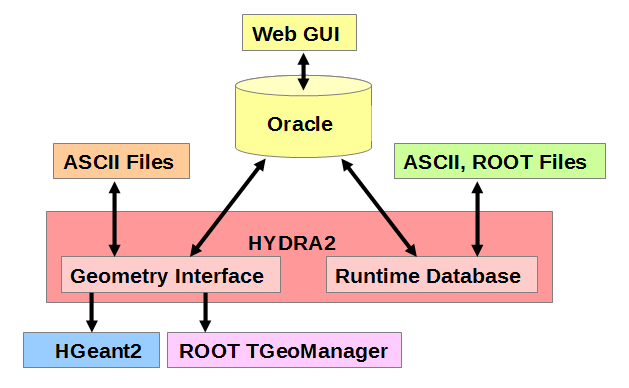
\includegraphics[scale=0.45]{hydra2_rtdb.png}
  \caption[Parameter interfaces]{Parameter interfaces} \label{fig:parameterInterfaces}
\end{figure}

All parameters are permanently stored in the \textbf{HADES Oracle database} (chapter~\ref{ch:oracle}). It stores all 
actually valid and historic parameters for all beam times and simulations.\\
Web-based interfaces (\textbf{WebDB}) provide additional access to the data in Oracle without running an analysis.\\

The design of the database tables is not the same for all parameter containers.\\
Some of the tables are closely related to the technical structure of the detectors, as they hold not only parameters 
needed by the analysis, but also information about the electronic setup and the cabling. As a result the data 
are spread over a large number of tables.\\
Other containers with large amounts of data in a tree like structure are stored in a certain fixed schema 
(\textbf{tree-style parameter containers}).\\
All these containers need special interface functions to retrieve and store the data.\\
But most parameter containers developed in the last years use a fixed layout and data are read and stored with a 
base class interface (\textbf{condition-style parameter containers}).\\

Almost all parameter containers need a \textbf{version management} to keep track of changes 
(see~\ref{sec:oraVersionmanagement}).\\
One version is valid for one or more event files characterized by the run id. For the same run, even several versions 
of parameters might exist, for example a first version of calibration parameters, a second version after a more 
detailed analysis, etc. It must be possible to read also these historic data in the analysis.\\

Some parameters even come with different flavors, called \textbf{context}, for example wide cuts or strong cuts.\\

For daily work one needs an additional storage medium for the runtime database: \textbf{ROOT files} have been 
foreseen to store parameter sets temporarily as objects.\\
For several reasons a local version management has been implemented:
\begin{itemize}
 \item To run many jobs in parallel on the batch farm.
 \item To hold the parameters locally to avoid net traffic.
 \item To distribute the parameters within the collaboration when the direct access to Oracle is not possible or too
   slow or when the newest data are not yet stored in Oracle.
\end{itemize}
The ROOT file may contain all parameters to run the analysis of a dedicated list of runs (subset of the parameter  versions in Oracle).\\ 

To have an easy way to edit or create parameters, an interface to \textbf{ASCII files} has been implemented as well.
The aim was not to store all data temporarily in ASCII files, but to have an easy way to change parameters with an 
editor or to compare different versions. A local version management was \textbf{not} implemented.
